% TEMPLATE for Usenix papers, specifically to meet requirements of
%  USENIX '05
% originally a template for producing IEEE-format articles using LaTeX.
%   written by Matthew Ward, CS Department, Worcester Polytechnic Institute.
% adapted by David Beazley for his excellent SWIG paper in Proceedings,
%   Tcl 96
% turned into a smartass generic template by De Clarke, with thanks to
%   both the above pioneers
% use at your own risk.  Complaints to /dev/null.
% make it two column with no page numbering, default is 10 point

% Munged by Fred Douglis <douglis@research.att.com> 10/97 to separate
% the .sty file from the LaTeX source template, so that people can
% more easily include the .sty file into an existing document.  Also
% changed to more closely follow the style guidelines as represented
% by the Word sample file. 

% Note that since 2010, USENIX does not require endnotes. If you want
% foot of page notes, don't include the endnotes package in the 
% usepackage command, below.

% This version uses the latex2e styles, not the very ancient 2.09 stuff.
\documentclass[letterpaper,twocolumn,10pt]{article}
\usepackage{usenix,epsfig,endnotes}
\begin{document}

%don't want date printed
\date{}

%make title bold and 14 pt font (Latex default is non-bold, 16 pt)
\title{
  \Large \bf Forecasting Attributes of Tropical Cyclones\\
             Using Robust Locally Weighted Regression
}

\author {
  {\rm Ali Yahya}\\
  Stanford University
  % copy the following lines to add more authors
  % \and
  % {\rm Name}\\
  %Name Institution
} % end author

\maketitle

% Use the following at camera-ready time to suppress page numbers.
% Comment it out when you first submit the paper for review.
% \thispagestyle{empty}


\subsection*{Abstract}
Critical sensor data about the state of an active tropical cyclone is often
incomplete or inconsistent. We present a forecast model that attempts to capture
a fundamental understanding of the relationships between a storm's different
numerical attributes. The model can thereby help verify or reconstruct corrupted
data about any given tropical cyclone. The forecast model we present is based on
a supervised machine learning algorithm known as LOESS which implements robust
locally weighted regression in $n$-dimensional space, where $n$ is the number
of attributes of the storm under consideration. The model presented yields good
results with error margins of less than 10\% for attributes that exhibit a high
degree of correlation with other attributes in the model.



\section{Introduction}

Tropical cyclones are highly structured storm systems that are characterized by
numerous thunderstorms, strong winds, and heavy rain that revolve around a large
low-pressure center. Because of the high degree of structure in tropical
cyclones, their data model is well defined and relatively self-contained.
Consequently, forecast models that treat tropical cyclones as systems in
isolation---that is, without consideration for collateral or larger scale
factors---can be more successful than similar models applied to less structured
storm systems.

\subsection{Patterns in Hurricane Data Models}
At any given moment, any one tropical cyclone and its present behavior can be
almost entirely described with values for a relatively small set of attributes.
One important subset of those attributes could include: minimum central
pressure, maximum wind speeds, latitude, longitude, radius of eyewall, radius of
maximum wind speed, radius of outer closed isobar, pressure of outer closed
isobar, among others. Moreover, previous studies have indicated that said
attributes not only represent a reasonably complete snapshot of a tropical
cyclone's behavior but also that they are highly correlated with each
other~\cite{SHIPS}.

In this paper, we analyze data for approximately over 1,000 hurricanes in the
Atlantic and Eastern North Pacific Basins. For each hurricane in the dataset, we
considered between 10 and 30 six-hourly snapshots of the storms attributes. We
point out a number of statistically significant correlations between seven
attributes that generally pertain to tropical cyclones~\cite{SHIPS}.

Further, we formalize our observations and present a forecast
model, based on locally weighted linear regression, that allows meteorologists
to use historical storm data to extrapolate the value of a single corrupted data
attribute in the data model of a storm, given correct values for a sufficient
number of other attributes.

\subsection{Motivation:\\Extrapolating Sensor Data}
Often times, at the most critical moment of a storm's development, sensor data
about its state can be incomplete or fraught with inconsistencies. In situations
like that, a forecast model that is based on a fundamental understanding of the
relationships between a storm's different attributes can help verify or 
reconstruct a dataset of an ongoing storm.

Additionally, a forecast model that sheds light on the interactions between
the different attributes in a storm's data model, enables meteorologists to
better predict the side-effects of changes to any one of those attributes.
Consequently, a successful forecast model for tropical cyclones may not only
improve the accuracy of warnings issued, but also their qualitative preciseness.

For instance, although it's fairly well understood that a increase in minimum
central pressure will result in a decrease of maximum wind speeds, it is also
important to consider a more subtle effect: A decrease in minimum central
pressure will indeed result in lower wind speeds, but because of the law of
Conservation of Angular Momentum, the radius around which maximum wind speeds
revolve will also increase. Therefore, the resulting storm surge and size of the
area of devastation will be different than with lower pressure and higher wind
speeds. Understanding exactly how such factors are likely to be different is
critical for the effectiveness of a tropical cyclone warning system.


\section{Patterns Observed}

As a preliminary step to crafting a unified forecast model, we present a number
of statistically significant pairwise correlations that were observed from
plots of data from \emph{The Tropical Cyclone Extended Best Track
Dataset}~\cite{BestTrackDataset}. The following attributes of approximately 
1,000 tropical cyclones were observed:
\begin{itemize}
  \item latitude
  \item longitude
  \item maximum wind speed
  \item minimum central pressure
  \item radius of maximum wind speed
  \item pressure of outer closed isobar
  \item radius of outer closed isobar
\end{itemize}
In the following sub-sections, we present a summary of the four most important
pairwise correlations observed.


\subsection{Pressure vs. Wind Speeds}

The most clearly expressed pairwise relationship in the data was that between
tropical cyclones' minimum central pressure and it's corresponding maximum wind
speeds. As illustrated by Figure \ref{pressure_vs_speed}, there is
a strong negative correlation between the two attributes.
\begin{figure}[h!]
  \centering
  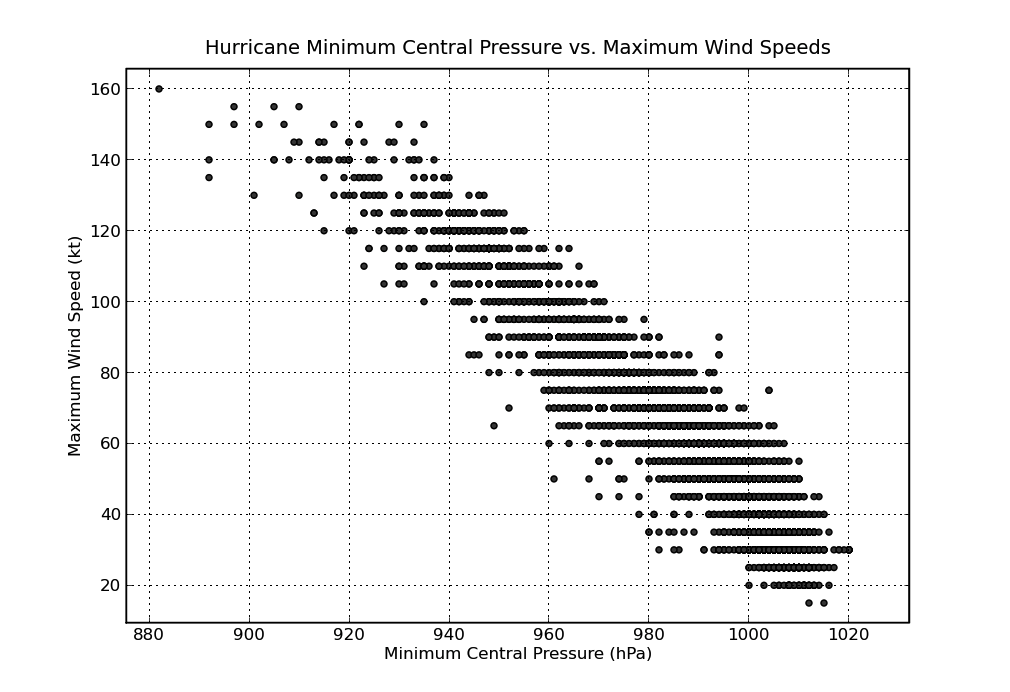
\includegraphics[scale=0.31]{pressure_vs_speed.png}
  \caption{Pressure vs. Wind Speeds}
  \label{pressure_vs_speed}
\end{figure}

Because the magnitude of the pressure gradient in the atmosphere is the primary
driver of wind speeds~\cite{MeteorologyToday}, it is not unexpected that a storm
with a lower pressure center would produce higher wind speeds.


\subsection{Pressure vs. Max. Wind Speed Radius}
A more subtle pairwise interaction (that was alluded to before) is that between
tropical cyclones' minimum central pressure and the radius around which the 
cyclone's maximum wind speeds revolve. Figure \ref{pressure_vs_radius}
illustrates a statistically significant positive correlation between the two
attributes.
\begin{figure}[h!]
  \centering
  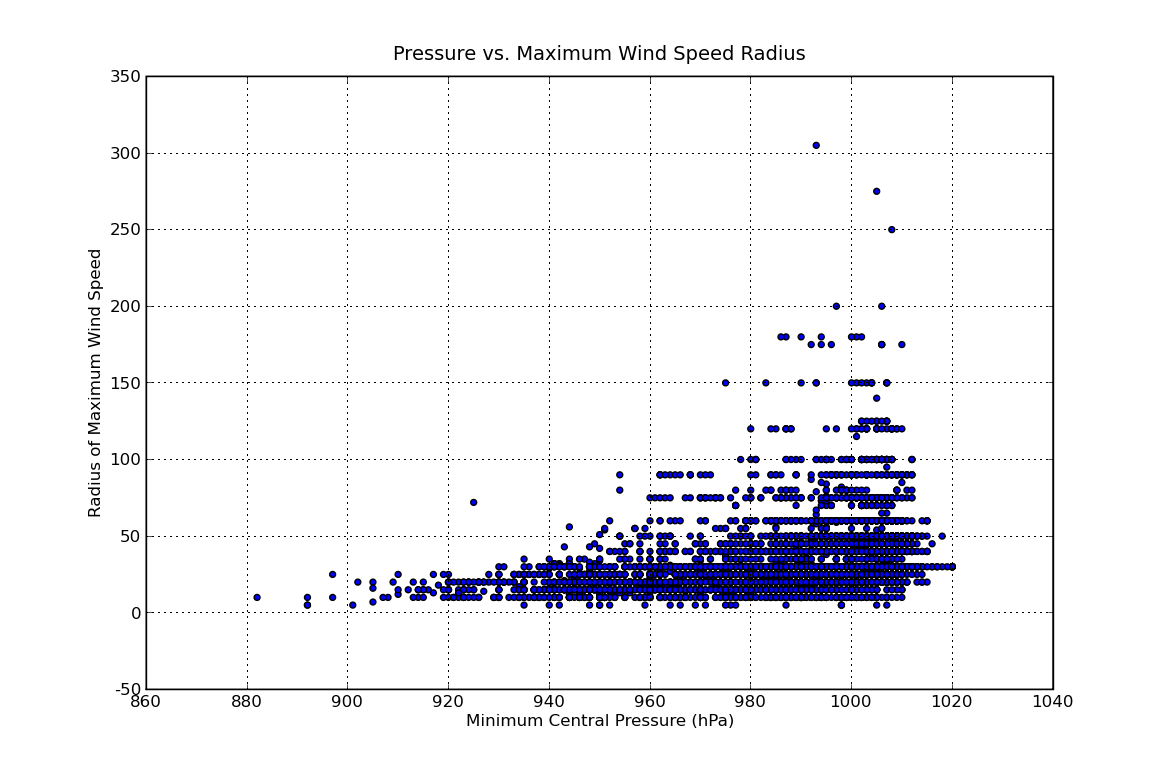
\includegraphics[scale=0.27]{pressure_vs_radius.png}
  \caption{Pressure vs. Max. Wind Speed Radius}
  \label{pressure_vs_radius}
\end{figure}

Note that, because of the relationship between pressure and wind speed described
in the previous section, a higher central pressure is correlated with slower
wind speeds. Because of the law of Conservation of Angular Momentum, slower wind
speeds are in-turn correlated with larger wind speed radii. Consequently, a
tropical cyclone's minimum central pressure is positively correlated with the
radius of the storm's maximum wind speeds.


\subsection{Maximum Wind Speed vs.\\Maximum Wind Speed Radius}
\begin{figure}[h!]
  \centering
  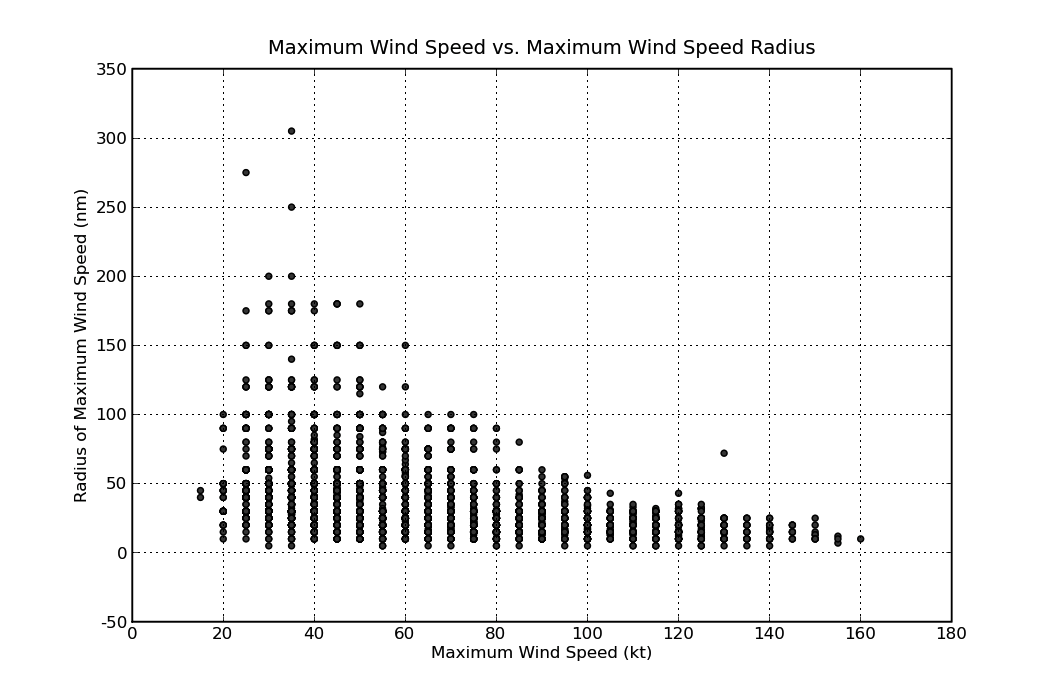
\includegraphics[scale=0.31]{speed_vs_radius.png}
  \caption{Max. Wind Speed vs. Wind Speed Radius}
  \label{speed_vs_radius}
\end{figure}
A direct corollary of the relationship described in the previous section, is the
negative correlation between maximum wind speed and maximum wind speed radius.
The relationship is illustrated by Figure \ref{speed_vs_radius}. Note that as
maximum wind speeds increase, the maximum wind speed radius tends to decrease.

\subsection{Longitude vs. Wind Speed}
Finally, Figure \ref{longitude_vs_speed} reveals that as hurricanes in the
Atlantic basin move westward, their maximum wind speeds tend to increase.
However, once storms reach a certain longitude (i.e. approximately $90^\circ$
West), wind speeds dramatically drop. This can be attributed to probable
landfall.
\begin{figure}[h!]
  \centering
  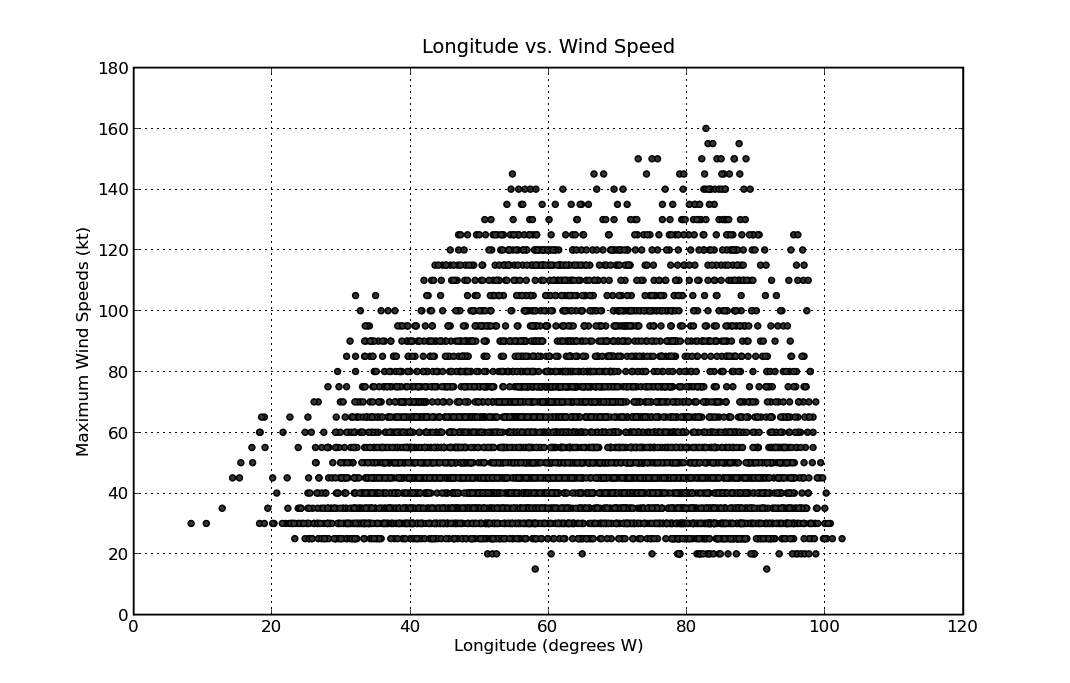
\includegraphics[scale=0.31]{longitude_vs_speed.png}
  \caption{Longitude vs. Max. Wind Speeds}
  \label{longitude_vs_speed}
\end{figure}

As a tropical cyclone travels over land, its primary source of energy, warm
evaporating water, is no longer available. Consequently, the storm weakens and
eventually dissipates. Note that the cluster of data points with wind speeds of
around $120$ knots at longitudes of around $100^\circ$ occurred over the Gulf of
Mexico.

\section{Crafting a Numerical Weather Model}

We present a numerical model that captures the many-to-many relationships
between the different attributes that can be used to describe a tropical
cyclone's behavior. The model is based on a supervised machine learning
algorithm known as LOESS~\cite{LOESS}. The algorithm implements robust locally
weighted regression in $n$-dimensional space, where $n$ is the number of
attributes taken into account by the model. In contrast to the manual, pair-wise
analysis used to identify a few trends in the data in the previous section, the
numerical model succeeds at capturing the relationship between each attribute
and every other attribute in the model.

\subsection{Training the Learning Algorithm}
Predictions made by the numerical model about any particular tropical cyclone
are based on a database containing historical data of similar tropical cyclones
that have occurred in the past. For this reason, LOESS is a supervised learning
algorithm, as it requires training data whose correctness is, in a sense,
\emph{supervised}.

The training data used with our implementation of the algorithm comes from 
the same dataset that we used in the previous section~\cite{BestTrackDataset}.

\subsection{Estimating the Model's Parameters}




\bibliographystyle{acm}
\bibliography{references}

% \theendnotes

\end{document}
